% \chapter{The Frenet Frame} \label{chap:frenet}
% %
% An alternative to the director frame is the Frenet frame, which is widely seen as the natural frame for topology and differential geometry. In the Frenet frame a curve is described by a tangent~$\boldsymbol{\tau}$, a unit normal~$\boldsymbol{\nu}$ and a binormal~$\boldsymbol{\beta}$ vectors, which satisfy the following
% %
% \begin{equation}
% \boldsymbol{\tau} = \boldsymbol{d}_{3} \quad \boldsymbol{\nu} = \left| \boldsymbol{\tau}^{\prime} \right|  \quad \mbox{and} \quad \boldsymbol{\beta} = \boldsymbol{\tau}\times\boldsymbol{\nu}, \label{eq:frenet_1}
% \end{equation}
% %
% where $\kappa$ are is curvature defined by
% %
% \begin{align}
% \kappa^{2} & = u_{1}^{2} + u_{2}^{2}.
% \end{align}
% %
% From~\eqref{eq:frenet_1} it follows that
% %
% \begin{align}
% \boldsymbol{\beta}^{\prime} & = - \tau_{s} \boldsymbol{\nu},
% \end{align}
% %
% where $\tau_{s}$ is the geometric torsion of the curve. Finally
% %
% \begin{align}
% \boldsymbol{\nu}^{\prime} & = \tau_{s} \boldsymbol{\beta} - \kappa \boldsymbol{\tau}.
% \end{align}
% %
% Hence the evolution equations are Hamiltonian, having a skew-symmetric structure matrix given by
% %
% \begin{align}
% \left( \begin{array}{c}
% \boldsymbol{\tau} \\
% \boldsymbol{\nu} \\
% \boldsymbol{\beta}
% \end{array} \right)^{\prime} & = 
% \left( \begin{array}{ccc}
% \boldsymbol{0} & -\kappa\mathbb{I}_{3} & \boldsymbol{0} \\
% \kappa\mathbb{I}_{3} & \boldsymbol{0} & \tau_{s}\mathbb{I}_{3} \\
% \boldsymbol{0} & -\tau_{s}\mathbb{I}_{3} & \boldsymbol{0}
% \end{array} \right)
% \left( \begin{array}{c}
% \boldsymbol{\tau} \\
% \boldsymbol{\nu} \\
% \boldsymbol{\beta} 
% \end{array} \right).
% \end{align}
% %
% \par
% The Frenet frame may be related to the director frame by a rotation. Following~\cite[\S 253]{Love44} the rotation angle is given by $\pi\slash 2 - f$, where
% %
% \begin{align}
% \tan f & = -\frac{u_{2}}{u_{1}}. \label{eq:register}
% \end{align}
% %
% The angle $f$ is often called the register. The local internal twist can be defined as $\tau_{i}= f^{\prime}$. The local twist $\tau=u_{3}$ may be expressed as the sum of the torsion of the centreline and the internal twist, that is
% %
% \begin{align}
% \tau & = \tau_{i} + \tau_{s}.
% \end{align}
% %
% The principal advantage of the Frenet frame is that for a helix the forces and moments are both orthogonal to the normal $\boldsymbol{\nu}$ and that the curves can be characterised by having constant torsion and curvature. 
% %
\chapter{Parameterisation} \label{chap:parameterisation}
%
In order to convert any quantities in the spatial frame to the director frame a form of parameterisation is needed that perserves the structure of the equations under the action of the symmetry group ${SO}\left(3\right)$ as required in~\eqref{eq:frame}. There are two principal coordinate charts which are commonly employed: the Euler angles and the Euler parameters.  In this appendix both forms of parameterisation are outlined. The Euler angles are analytically simple and have a distinct physical interpretation, making them amenable to analytical methods, yet have an inherent polar singularity which, coupled with appearance of trigonometric functions precludes them from complex numerical calculation. However, under suitable conditions the singularity may be moved to infinity, c.f.~\eqref{eq:torque_condition}. The Euler parameters are a set of unit quarternions and have little tangible physical meaning. Indeed, with exception of Kehrbaum~\cite{Kehrbaum97b}, there is little analytical work in this formulation relating to rods. The Euler parameters have the property of double covering which removes the singularity and are numerically straightforward to implement\footnote{Goldstein, writing without the knowledge of today's computation power in an earlier edition of his text on classical mechanics alludes to the supposed redundancy of quarternions by dismissively referring to them as ``musty mathematics'' but this quote has been removed from the latest edition~\cite{Goldstein02}.}.
%
\par
There are other forms of parameterisation, most notably the Deprit-Andoyer variables as used in~\cite{Mielke88}. They are well chosen choices for the co-terminal rotations and say no more than the Euler Angles. The Serret-Andoyer equations can be derived either by solving a Hamilton-Jacobi in the Euler angles or constructed geometrically as a series of rotations. 
%
\section{Euler Angles} \label{sec:euler_angles}
%
The Euler angles are defined by three consecutive rotations which convert quantities in the spatial frame to the director frame. For consistency we shall let $\left(x^{\left(0\right)}, y^{\left(0\right)}, z^{\left(0\right)}\right)$ denote components of a vector in the spatial frame $\left\{ \boldsymbol{e}_{1},\boldsymbol{e}_{2},\boldsymbol{e}_{3} \right\}$ and let $\left(x^{\left(3\right)}, y^{\left(3\right)}, z^{\left(3\right)} \right)$ denote components of a 3-tuple written in the director frame $\left\{ \boldsymbol{d}_{1}, \boldsymbol{d}_{2}, \boldsymbol{d}_{3} \right\}$. Components of $3$-tuples in intermediate bases will be denoted with accordingly. There is no standard notation for Euler angle formulations\footnote{There are twelve distinct Euler angle sequences} but following from Heijden~\cite{Heijden00a} and adopting the conventions of the so-called British school of Love, Whittaker and Pars \emph{et al.}, the transformation can be parameterised by the following three rotations:
%They do not form an atlas as they do not give a global description of a system.
\begin{itemize}\addtolength{\itemsep}{-0.4\baselineskip}
\item[(i)] A rotation $R_{1}\left(\phi\right)$ about $z_{0}$ by $\phi$ mapping $x^{\left(0\right)}$ and $y^{\left(0\right)}$ onto $x^{\left(1\right)}$ and $y^{\left(1\right)}$ respectively.
\item[(ii)] A rotation $R_{2}\left(\theta\right)$ about $x_{1}$ by $\theta$ mapping $y^{\left(1\right)}$ and $z^{\left(1\right)}$ onto and $y^{\left(2\right)}$ and $z^{\left(2\right)}$.
\item[(iii)] A rotation $R_{3}\left(\psi\right)$ about $z^{\left(2\right)}$ by $\psi$ mapping $x^{\left(2\right)}$ and $y^{\left(2\right)}$ onto $x^{\left(3\right)}$ and $y^{\left(3\right)}$.
\end{itemize}
%
\begin{figure} 
\begin{center}
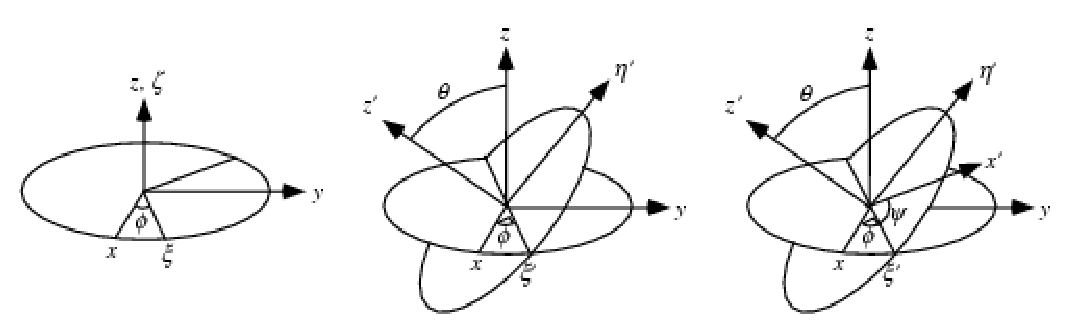
\includegraphics[scale=0.75]{Images/EulerAngles_600.ps}
\caption[The Euler angles]{\baselineskip=1.0\normalbaselineskip%
The three consecutive rotations $\phi$, $\theta$ and $\psi$ which produces the Euler angles. \label{fig:angles}}
\end{center}
\end{figure}
% 
Explicitly, the rotation $R_{1}$ acts by
%
\begin{align*}
\left( 
\begin{array}{c}
x^{\left(1\right)} \\
y^{\left(1\right)} \\
z^{\left(1\right)}
\end{array} 
\right)
& = \left( 
\begin{array}{ccc}
\sin\phi & \cos\phi & 0 \\
\cos\phi & -\sin\phi & 0 \\
0 & 0 & 1 
\end{array} 
\right)
\left( 
\begin{array}{c}
x^{\left(0\right)} \\
y^{\left(0\right)} \\
z^{\left(0\right)} 
\end{array} \right),
\end{align*}
%
the second rotation $R_{2}$ is given by
%
\begin{align*}
\left( 
\begin{array}{c}
x^{\left(2\right)} \\
y^{\left(2\right)} \\
z^{\left(2\right)}
\end{array} 
\right)
& = \left( 
\begin{array}{ccc}
1 & 0 & 0 \\
0 & \cos\theta & -\sin\theta \\ 
0 & \sin\theta & \cos\theta 
\end{array} 
\right)
\left( 
\begin{array}{c}
x^{\left(1\right)} \\
y^{\left(1\right)} \\
z^{\left(1\right)} 
\end{array} 
\right)
\end{align*}
%
and the final rotation $R_{3}$ is given by
%
\begin{align*}
\left( 
\begin{array}{c}
x^{\left(3\right)} \\
y^{\left(3\right)} \\
z^{\left(3\right)}
\end{array} 
\right)
= \left( 
\begin{array}{ccc}
-\sin\psi & \cos\psi & 0 \\
\cos\psi & \sin\psi & 0 \\ 
0 & 0 & 1 
\end{array} 
\right)
\left( 
\begin{array}{c}
x^{\left(2\right)} \\
y^{\left(2\right)} \\
z^{\left(2\right)} 
\end{array} 
\right).
\end{align*}
%
Thus, evaluating the rotations consecutively gives the matrix 
%
\begin{align*}
R\left( \theta, \psi, \phi \right) & = R_{1}\left(\phi\right) R_{2}\left(\theta\right) R_{3}\left(\psi\right),
\end{align*}
%
which, by direct calculation yields
%
\begin{align}
R & = 
\left(
\begin{array}{ccc}
\cos\theta\cos\phi\cos\psi-\sin\phi\sin\psi & \cos\theta\cos\phi\sin\psi+\cos\psi\sin\phi & -\sin\theta\cos\phi \\
-\cos\theta\sin\phi\cos\psi-\cos\phi\sin\psi & -\cos\theta\sin\phi\sin\psi+\cos\phi\cos\psi & \sin\theta\sin\phi \\
\sin\theta\cos\psi & \sin\theta\sin\psi & \cos\theta
\end{array}
\right).
\label{eq:euler_matrix}
\end{align}
%
The set of rotations in displayed in figure~\ref{fig:angles}. The parameterisation of the directors is given explicitly by
%
\begin{subequations}
\label{eq:euler_angles}
\begin{align}
\boldsymbol{d}_{1}\left(\theta,\phi,\psi\right) & = 
\left(
\begin{array}{c}
\cos\psi\cos\theta\cos\phi - \sin\psi\sin\phi \\
\cos\psi\cos\theta\sin\phi + \sin\psi\cos\phi \\
-\cos\psi\sin\theta
\end{array}
\right), \label{eq:angles_d1} \\
\boldsymbol{d}_{2}\left(\theta,\phi,\psi\right) & = 
\left(
\begin{array}{c}
-\sin\psi\cos\theta\cos\phi + \sin\psi\cos\phi \\
-\sin\psi\cos\theta\sin\phi + \cos\psi\cos\phi \\
\sin\psi\sin\theta
\end{array}
\right), \label{eq:angles_d2} \\
\boldsymbol{d}_{3}\left(\theta,\phi\right) & = 
\left(
\begin{array}{c}
\sin\theta \cos\phi \\
\sin\theta \sin\phi \\
\cos\theta 
\end{array}
\right).\label{eq:angles_d3}
\end{align}
\end{subequations}
%
Here $\theta$ measures the displacement from an initially straight rod, $\psi$ is the azimuthal angle about a fixed axis and $\phi$ is the twist angle about the centreline of the rod. In the terminology of rigid body mechanics $\theta$ is the nutation angle, $\psi$ is the precession angle and $\phi$ is the spin angle. It is evident from the construction of $R$ that when there is no nutation that spin and precession are no longer independent.
%
\section{Euler Parameters} \label{sec:euler_parameters}
%
If a unit vector in the spatial frame, $\boldsymbol{k}$, is rotated by an angle $\Phi$, then the Euler parameters may be defined as 
%
\begin{equation}
\begin{array}{rl}
q_{j} & = \boldsymbol{k} \cdot \boldsymbol{e}_{j} \sin \left( \Phi \slash 2 \right), \quad j=1,2,3. \\
q_{4} & = \cos \left( \Phi \slash 2 \right),
\end{array}
\label{eq:def_ep}
\end{equation}
%
subject to the normalisation condition
%
\begin{align}
q_{1}^{2} + q_{2}^{2} + q_{3}^{2} + q_{4}^{2} & = 1.
\label{eq:euler_constraint}
\end{align}
%
This is equivalent to making the substitutions
%
\begin{equation*}
q_{1} = \cos \frac{\psi+\phi}{2} \cos \frac{\theta}{2}, \quad q_{2} = \cos \frac{\psi-\phi}{2} \sin \frac{\theta}{2}, \quad q_{3} = \sin \frac{\psi-\phi}{2} \sin \frac{\theta}{2}
\end{equation*}
%
and
% 
\begin{equation*} 
q_{4} = \sin \frac{\psi+\phi}{2} \cos \frac{\theta}{2}
\end{equation*}
% 
into the matrix~\eqref{eq:euler_matrix}. Thus the rotation matrix $R$ is given by
% 
\begin{align}
R & = 
\left(
\begin{array}{ccc}
q_{1}^{2} - q_{2}^{2} - q_{3}^{2} + q_{4}^{2} & 2\left(q_{1}^{}q_{2}^{} - q_{3}^{}q_{4}^{}\right) & 2\left(q_{1}^{}q_{3}^{} + q_{2}^{}q_{4}^{}\right) \\
2\left(q_{1}^{}q_{2}^{} + q_{3}^{}q_{4}^{} \right) & q_{2}^{2} + q_{4}^{2} - q_{1}^{2} - q_{3}^{2} & 2\left(q_{2}^{}q_{3}^{} - q_{1}^{}q_{4}^{} \right) \\
2\left(q_{1}^{}q_{3}^{} - q_{2}^{}q_{4}^{} \right) & 2\left(q_{1}^{}q_{4}^{} - q_{2}^{}q_{3}^{} \right) & q_{3}^{2} + q_{4}^{2} - q_{1}^{2} - q_{2}^{2}
\end{array}
\right).
\end{align}
% 
In terms of Euler parameters the directors are given by 
%
\begin{subequations}
\label{eq:euler_parameters}
\begin{align}
\boldsymbol{d}_{1}^{} & = 
\left(
\begin{array}{c}
q_{1}^{2} - q_{2}^{2} - q_{3}^{2} + q_{4}^{2} \\
2\left(q_{1}^{}q_{2}^{} + q_{3}^{}q_{4}^{} \right) \\
2\left(q_{1}^{}q_{3}^{} - q_{2}^{}q_{4}^{} \right)
\end{array}
\right), \label{eq:parameters_d1} \\
\boldsymbol{d}_{2}^{} & = 
\left(
\begin{array}{c}
2\left(q_{1}^{}q_{2}^{} - q_{3}^{}q_{4}^{} \right) \\
q_{2}^{2} + q_{4}^{2} - q_{1}^{2} - q_{3}^{2} \\
2\left(q_{1}^{}q_{4}^{} - q_{2}^{}q_{3}^{} \right)
\end{array}
\right),\label{eq:parameters_d2} \\
\boldsymbol{d}_{3}^{} & = 
\left(
\begin{array}{c}
2\left(q_{1}^{}q_{3}^{} + q_{2}^{}q_{4}^{} \right) \\
2\left(q_{2}^{}q_{3}^{} - q_{1}^{}q_{4}^{} \right) \\
q_{3}^{2} + q_{4}^{2} - q_{1}^{2} - q_{2}^{2}
\end{array}
\right). \label{eq:parameters_d3}
\end{align}
\end{subequations}
% 
\par
If the quarternion ${q}$ corresponds to the rotation of $\boldsymbol{k}$ by $\Phi$ then $-{q}$ corresponds to the co-terminal rotation of $\boldsymbol{k}$ by $\Phi + 2\,\pi$. Hence $q$ and $-q$ give the same description of a coordinate chart and thus there is a homomorphic two-to-one relationship between representations with the Euler parameters and rotations. The homomorphism manifests itself as the spin-$\frac{1}{2}$ properties since for $q \mapsto q$ then $\Phi \mapsto \Phi + 4\,\pi$. This is because the Euler parameters provide a representation of the group $SU\left(2\right)$, rather than $SO\left(3\right)$.
% 
\begin{rem}
The curious property emerges that the Lie algebra $\mathfrak{su}\left(2\right)$ is isomorphic to the Lie algebra $\mathfrak{so}\left(3\right)$ but the associated Lie groups are not isomorphic. The isomorphism between the Lie algebras is exploited in the construction of the Lax pair and the homomorphism is exploited in the numerical calculations.
\end{rem}
% 
\begin{rem}
From the Euler angles a set of Cayley-Klein parameters $\left(\alpha, \beta, \gamma, \delta\right)$ can be constructed which are related to the Euler parameters through the relationship with the Pauli spin matrices~\cite{Goldstein02}
\begin{align}
\left( \begin{array}{cc}
\alpha & \beta \\
\gamma & \delta 
\end{array} \right) & = 
 i \left( p_{1}\sigma_{1} + p_{2}\sigma_{2} + p_{3}\sigma_{3} \right) + \mathbb{I}_{2} p_{4}.\nonumber
\end{align} 
Where the $\sigma_{i}$ are the Pauli spin matrices are given by
\begin{equation}
\sigma_{1} = \left( 
\begin{array}{cc}
0 & 1 \\
1 & 0
\end{array}
\right), \quad
\sigma_{2} = \left( 
\begin{array}{cc}
0 & -i \\
i & 0
\end{array}
\right) \quad \mbox{and} \quad
\sigma_{3} = \left( 
\begin{array}{cc}
1 & 0 \\
0 &-1
\end{array}
\right). \nonumber
\end{equation}
Each Pauli matrix represents an `observable' describing the spin of a spin-$\frac{1}{2}$ particle. An interesting property of spin-$\frac{1}{2}$ particles is that, as with the Euler parameters, they must be rotated by an angle of $4\pi$ in order to return to their original configuration.
\end{rem}
%
% \par
% Consider a rotation through an angle $\Phi$ about the direction of $\boldsymbol{k}$. Then there exists a rotation matrix $Q=Q\left(\Phi,\boldsymbol{k}\right)$ given by
% %
% \begin{align}
% Q & = \mathbb{I}_{2} \cos\frac{\Phi}{2} + i \boldsymbol{k}\cdot\boldsymbol{\sigma}\sin\frac{\Phi}{2} \nonumber \\
% & = e^{i \theta\slash{2}\boldsymbol{k}\cdot\boldsymbol{\sigma}}.
% \end{align}
% %
% Where the $\sigma_{i}$ are the Pauli spin matrices
% % 
% \begin{equation}
% \sigma_{1} = \left( 
% \begin{array}{cc}
% 0 & 1 \\
% 1 & 0
% \end{array}
% \right), \quad
% \sigma_{2} = \left( 
% \begin{array}{cc}
% 0 & -i \\
% i & 0
% \end{array}
% \right) \quad \mbox{and} \quad
% \sigma_{3} = \left( 
% \begin{array}{cc}
% 1 & 0 \\
% 0 &-1
% \end{array}
% \right). 
% \end{equation}
% %
% Thus $Q$ is a faithful representation of the group $SU\left(2\right)$.
% 
\par
The evolution of the Euler parameters can be derived by substituting the equations~\eqref{eq:euler_parameters} into~\eqref{eq:directors} to give
%
\begin{align}
\left( \begin{array}{c}
{q}_{1} \\
{q}_{2} \\
{q}_{3} \\
{q}_{4} 
\end{array} \right)^{\prime} 
% & = \frac{1}{2} 
% \left( \begin{array}{cccc}
% 0 & u_{3} & -u_{2} & u_{1} \\
% -u_{3} & 0 & u_{1} & u_{2} \\
% u_{2} & -u_{1} & 0 & u_{3} \\
% -u_{1} & -u_{2} & -u_{3} & 0 
% \end{array} \right)
% \left( \begin{array}{c}
% q_{1} \\
% q_{2} \\
% q_{3} \\
% q_{4} 
% \end{array} \right), \label{eq:ep_evolution_1} \\
& = \frac{1}{2} 
\left( \begin{array}{ccc}
p_{4} & -p_{3} & p_{2} \\
p_{3} & p_{4} & -p_{1} \\
-p_{2} & p_{1} & p_{4} \\
-p_{1} & -p_{2} & -p_{3}
\end{array} \right) 
\left( \begin{array}{c}
u_{1} \\
u_{2} \\
u_{3}
\end{array} \right). \label{eq:ep_evolution_2}
\end{align}
%
In one respect the normalisation condition~\eqref{eq:euler_constraint} can be seen as a Casimir as it is independent of any parameters.  However Casimirs can not be recovered from the evolution equation~\eqref{eq:ep_evolution_2} as the matrix is neither square nor skew-symmetric. Instead the normalisation condition can be interpreted as a geometric constraint. The Euler parameters exist on a submanifold (defined by the normalisation condition) on a higher dimensional `inflated' phase space designed to remove singularities~\cite{Dullin96}. Thus, the Euler parameters can be interpreted as being constrained to lie on the surface of a four-dimensional unit hyper-sphere. In the parlance of~\S\ref{chap:poisson} the normalisation condition is a geometric integral but not a Casimir. 
%
\par
The constraint is holonomic, thus by Frobenius's theorem inflating the phase space and adding a constraint does not affect the integrability of the parameterised system~\cite[pg. 624]{Abraham88}.
%
% For four-vectors the Euler parameters $pq = R(p)q$ where
%
% \begin{align}
% qp & = \left( \begin{array}{cccc}
% p_{4} & p_{3} & -p_{2} & p_{1} \\
% -p_{3} & p_{4} & p_{1} & p_{2} \\
% p_{2} & -p_{1} & p_{4} & p_{3} \\
% -p_{1} & -p_{2} & -p_{3} & p_{4} 
% \end{array}\right)
% \end{align}
% 
% The matrix $R\left(p\right)= -p_{1}B_{1} -p_{2}B_{2} - p_{3}B_{3} + p_{4}\mathbb{I}_{4}$. 